\documentclass[10pt,a4paper]{article}
\usepackage[utf8]{inputenc}
\usepackage[english]{babel}
\usepackage{amsmath}
\usepackage{amsfonts}
\usepackage{amssymb}
\usepackage{makeidx}
\usepackage{graphicx}
\usepackage[left=2cm,right=2cm,top=2cm,bottom=2cm]{geometry}
\author{Hao Peng}
\title{1CM30 - Service Supply Chains for Capital Goods
Spring 2014 \\
Exam Exercises - Set 4
Condition based maintenance \\
%Due date: Friday June 13 2014, 15:00 hours. \\
%Hand in a paper copy at the secretary (room PAV-E-5). \\
%Please define unambiguously all the variables you use and show your work clearly.
}
\begin{document}
\maketitle
\begin{enumerate}
\item The degradation of a production machine can be described by a DTM. The engineers collect the time to defect data in the lab by doing reliability testings. The time to defect data statistically suggest that the time to defect follows an exponential distribution with $\lambda=1$. The time unit is one month. The engineers also collect the data about the duration from the defect time point till failure in the lab. The delay time seems to be a constant value $0.5$, since the variance of the delay times are so small. 

For this production machine, we will apply a periodic inspection policy with a fixed inspection interval $\tau$. When we detect defects on the machine, we will overhaul the machine to prevent unexpected failures. Upon failures we will also overhaul the machine. 

The cost of a corrective overhaul is equal to EURO 3000. The cost of a preventive overhaul is equal to Euro 1000. The inspection cost is 10 Euro. 

\textbf{Apart from these costs, the time period in the defective state also incurs an extra energy cost with a rate 25 euro per month, since the production system will consume more energy in the defective state.} To illustrate the extra energy cost, please take a look at the figure given below. The duration of defective state in a renewal cycle multiplied by the extra energy rate 25 euro per month is equal to the extra energy cost for a renewal cycle. Since the duration of defective state in a renewal cycle is random (different from cycle to cycle), this extra energy cost in a renewal cycle is also random. We should take this extra energy cost into account while we are evaluating the expected cycle cost under different renewal events.
\begin{figure}[h!!!]  % ��ͼ���� i
  % Requires \usepackage{graphicx}
  \centering
  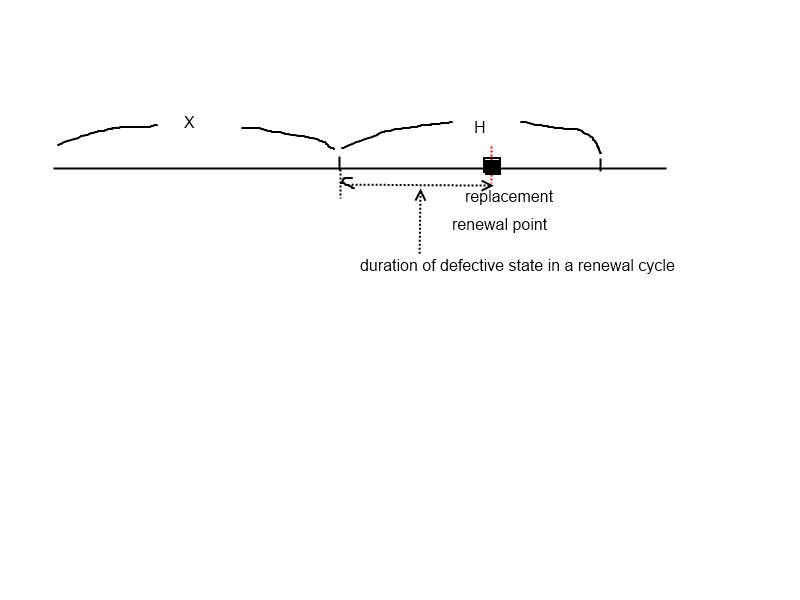
\includegraphics[width=6in]{exam1.png}\\
  \footnotesize
  \caption{ \footnotesize{ The Delay Time Model} }\label{DTM1}
\end{figure}


Determine the average costs of the periodic inspection policy as a function of $\tau$.


%\item The wear-out of a rotating part can be described by a a linear function, $X(t)=\theta t$. The time unit is one revolution. The wear-out can be determined by inspections on wear debris. Based on the wear-out mechanism, $\theta$ is dependent on the hardness of the material, the radius of the rotating part, and the force between rubbing surfaces. It is a random parameter among units. The engineers collect the degradation data of 80 units. For each unit, there's an estimated linear function through regression, which has an estimated $\hat{\theta}$. Then there are 80 $\hat{\theta}$ s. The engineers find out the distribution of $\theta$ is an exponential distribution with parameter $\hat{\lambda}= 1$, based on the 80 $\hat{\theta}$ s. The failure limit of the wear-out is given as $H=5000$.   
%
%\begin{itemize}
% \item Suppose the engineers set a warning limit of $C=4000$. What is the cdf of the first passage time over $C$ for this degrading component?
% \item Conditioned on the fact that the wear-out of the rotating component at 3500 revolutions is 4000, what is the conditional first passage time over $H$?   
% \end{itemize} 
%For this component, we will apply a periodic inspection policy with a fixed inspection interval $\tau$ and a control limit $C$. When the degradation level is above $C$ the component will get replaced. The degradation level can only be observed through inspections. Upon failures we will also replace the machine with a new one. The costs of a replacement are equal to EURO 3000. For a corrective maintenance action additional costs equal to EURO 1000 are incurred because of the disturbance of the production process that depends on the availability of the machine. The inspection cost is 10 Euro.
%
%Determine the average long run cost rate of the periodic inspection policy as a function of $\tau$ and $C$. 
\end{enumerate}
\end{document}